\begin{figure*}[!ht]
\center
%input
\centering
\begin{tabular}{p{0.125\linewidth}p{0.165\linewidth}p{0.165\linewidth}p{0.165\linewidth}p{0.165\linewidth}}
\centering{\textbf{Shape/Interest point}} & \centering Bicycle & \centering Kicking man & \centering Galleon & \centering Ant 
\end{tabular}
\subfloat{ 
\label{fig:mesh:input}
\makebox[0.15\linewidth]{\raisebox{0.07\linewidth}{(a) Input point clouds}} 
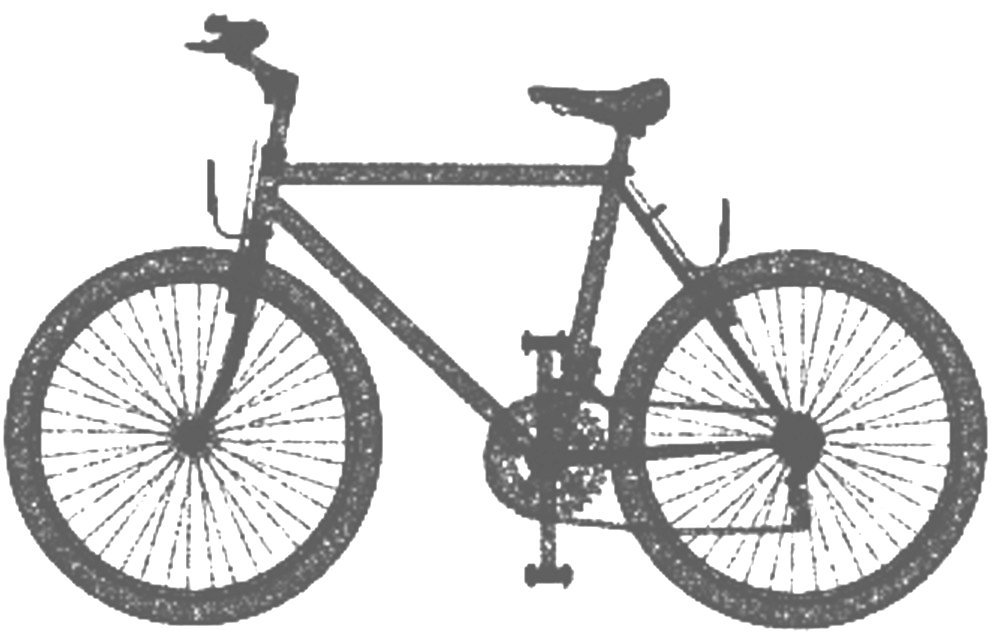
\includegraphics[width=0.175\linewidth]{./fig/eval/cycle_input.jpg} \hspace{0mm} 
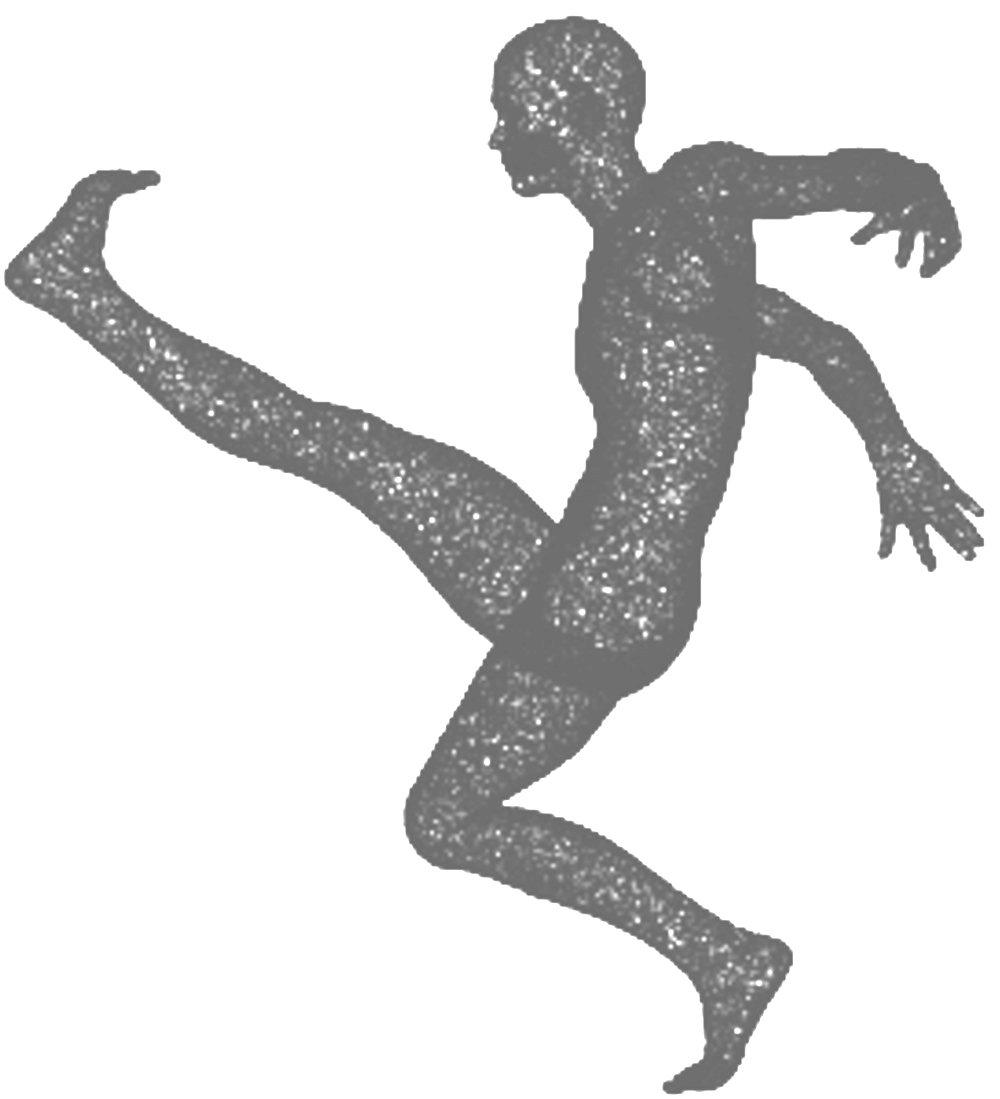
\includegraphics[width=0.155\linewidth]{./fig/eval/guy_input.jpg}  \hspace{0mm} 
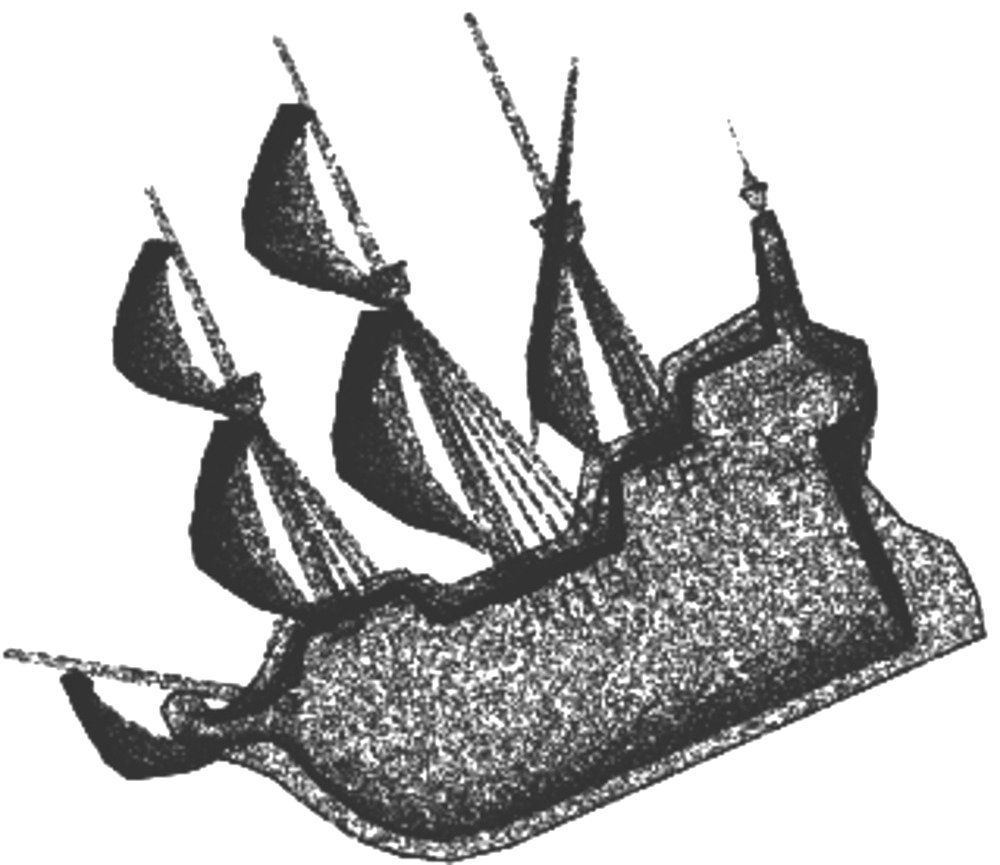
\includegraphics[width=0.175\linewidth]{./fig/eval/ship_input.jpg} \hspace{0mm}
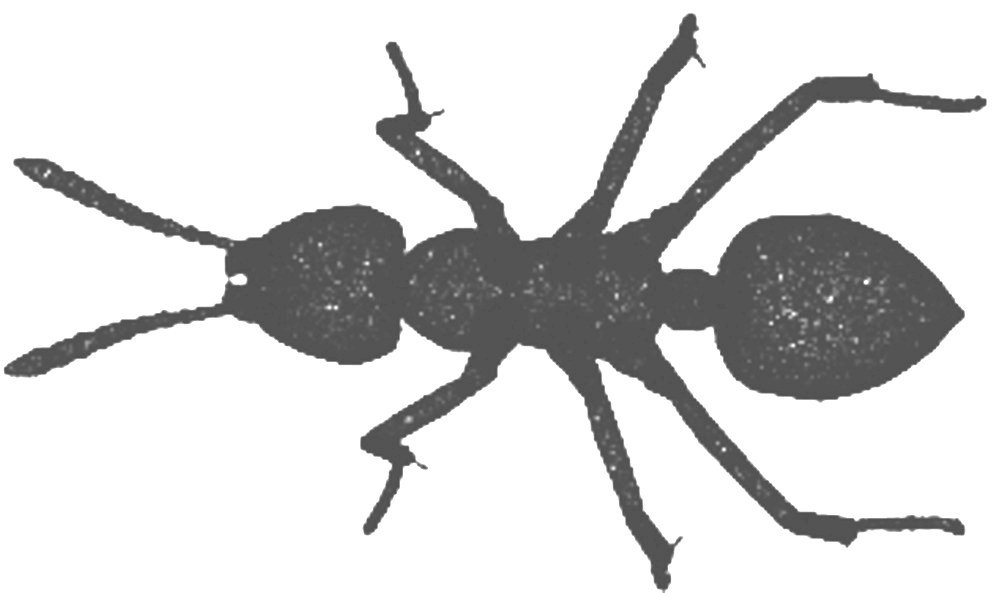
\includegraphics[width=0.175\linewidth]{./fig/eval/ant_input.jpg} 
} \vspace{-4mm} 
\\ 
% DoG
\subfloat{ 
\label{fig:mesh:dog}
\makebox[0.15\linewidth]{\raisebox{0.07\linewidth}{(b) DoG}} 
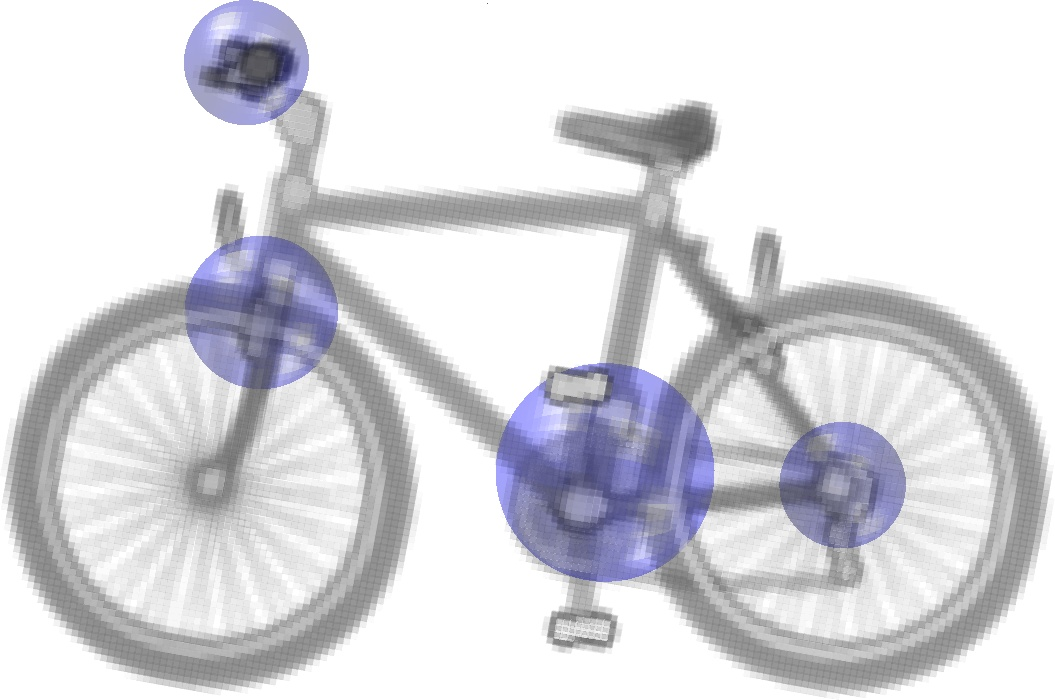
\includegraphics[width=0.175\linewidth]{./fig/eval/cycle_dog.jpg} \hspace{0mm} 
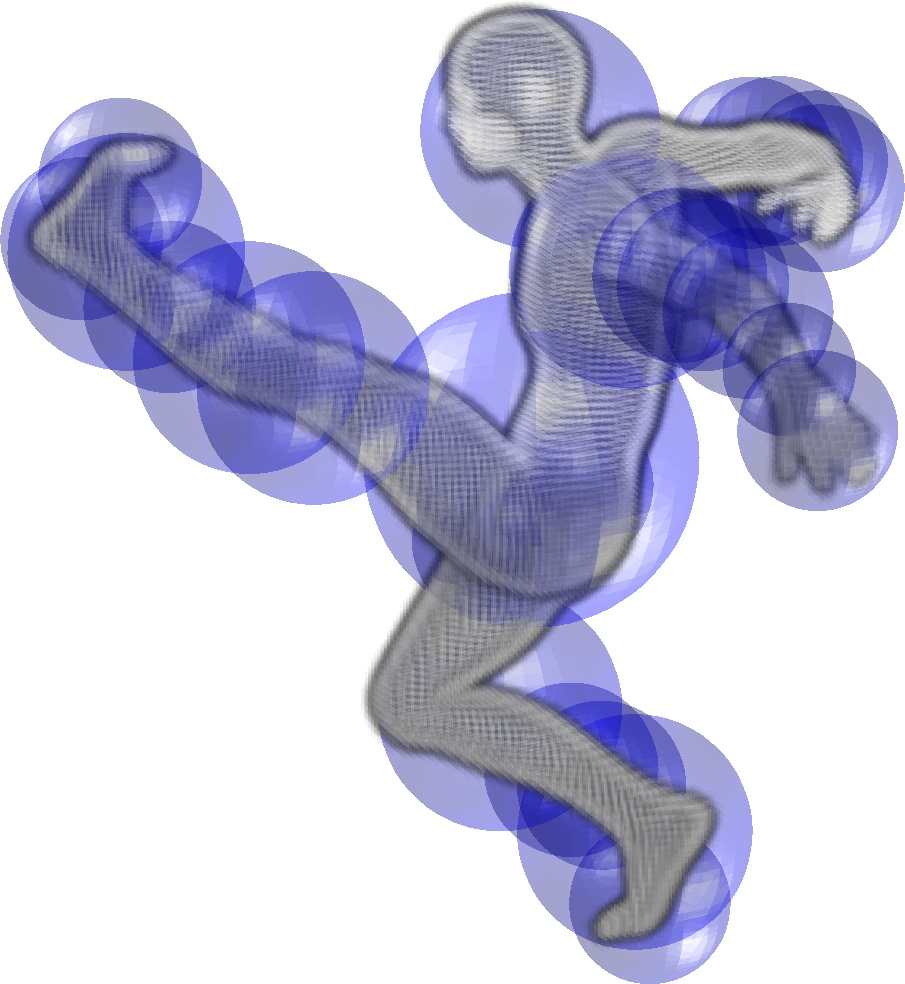
\includegraphics[width=0.155\linewidth]{./fig/eval/guy_dog.jpg}  \hspace{0mm}
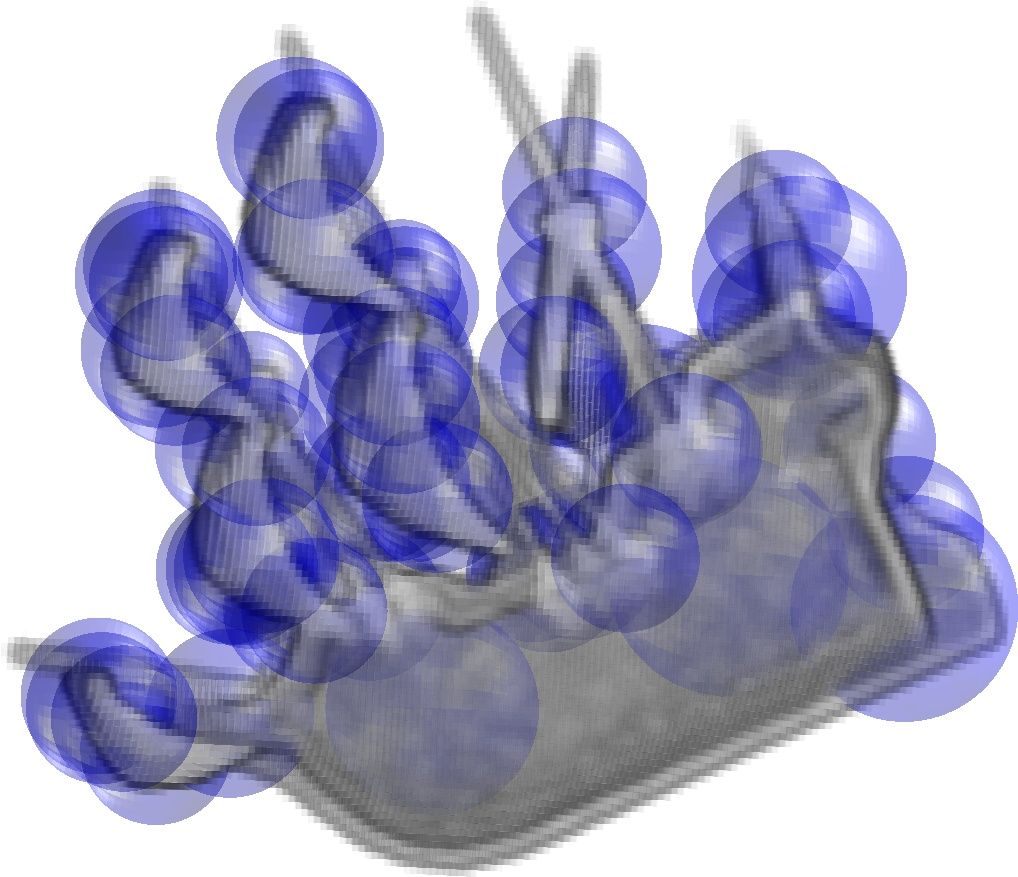
\includegraphics[width=0.175\linewidth]{./fig/eval/ship_dog.jpg} \hspace{0mm} 
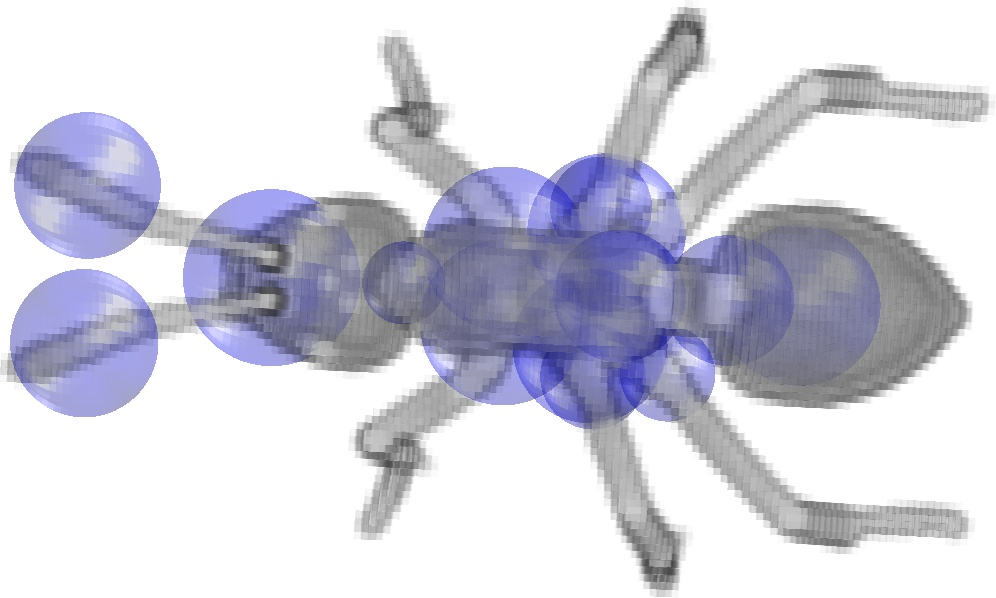
\includegraphics[width=0.175\linewidth]{./fig/eval/ant_dog.jpg} 
} \vspace{-4mm} 
\\ 
% SURF 
\subfloat{ 
\label{fig:mesh:surf}
\makebox[0.15\linewidth]{\raisebox{0.07\linewidth}{(c) SURF}}
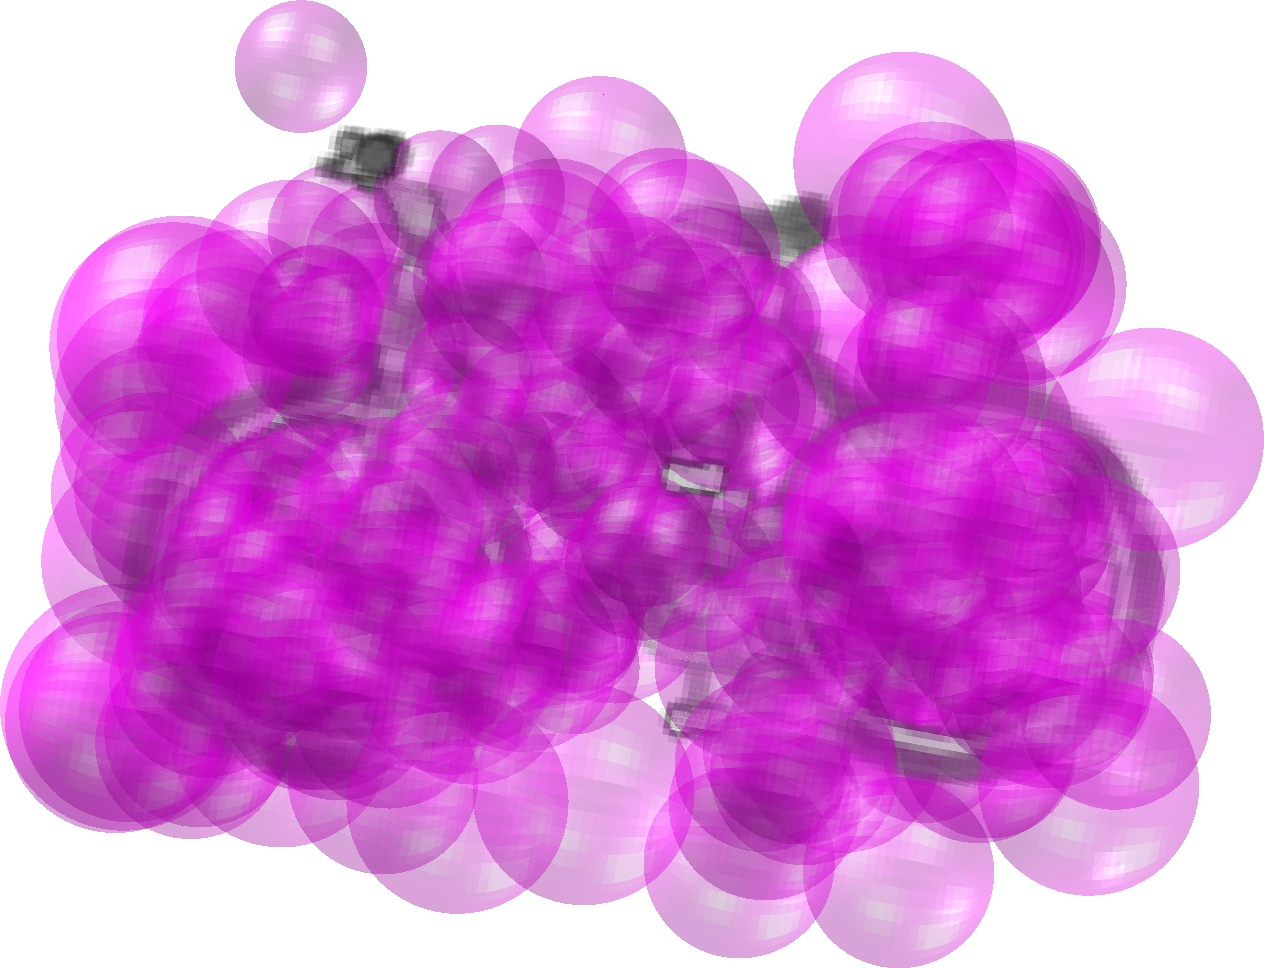
\includegraphics[width=0.175\linewidth]{./fig/eval/cycle_surf.jpg} \hspace{0mm}
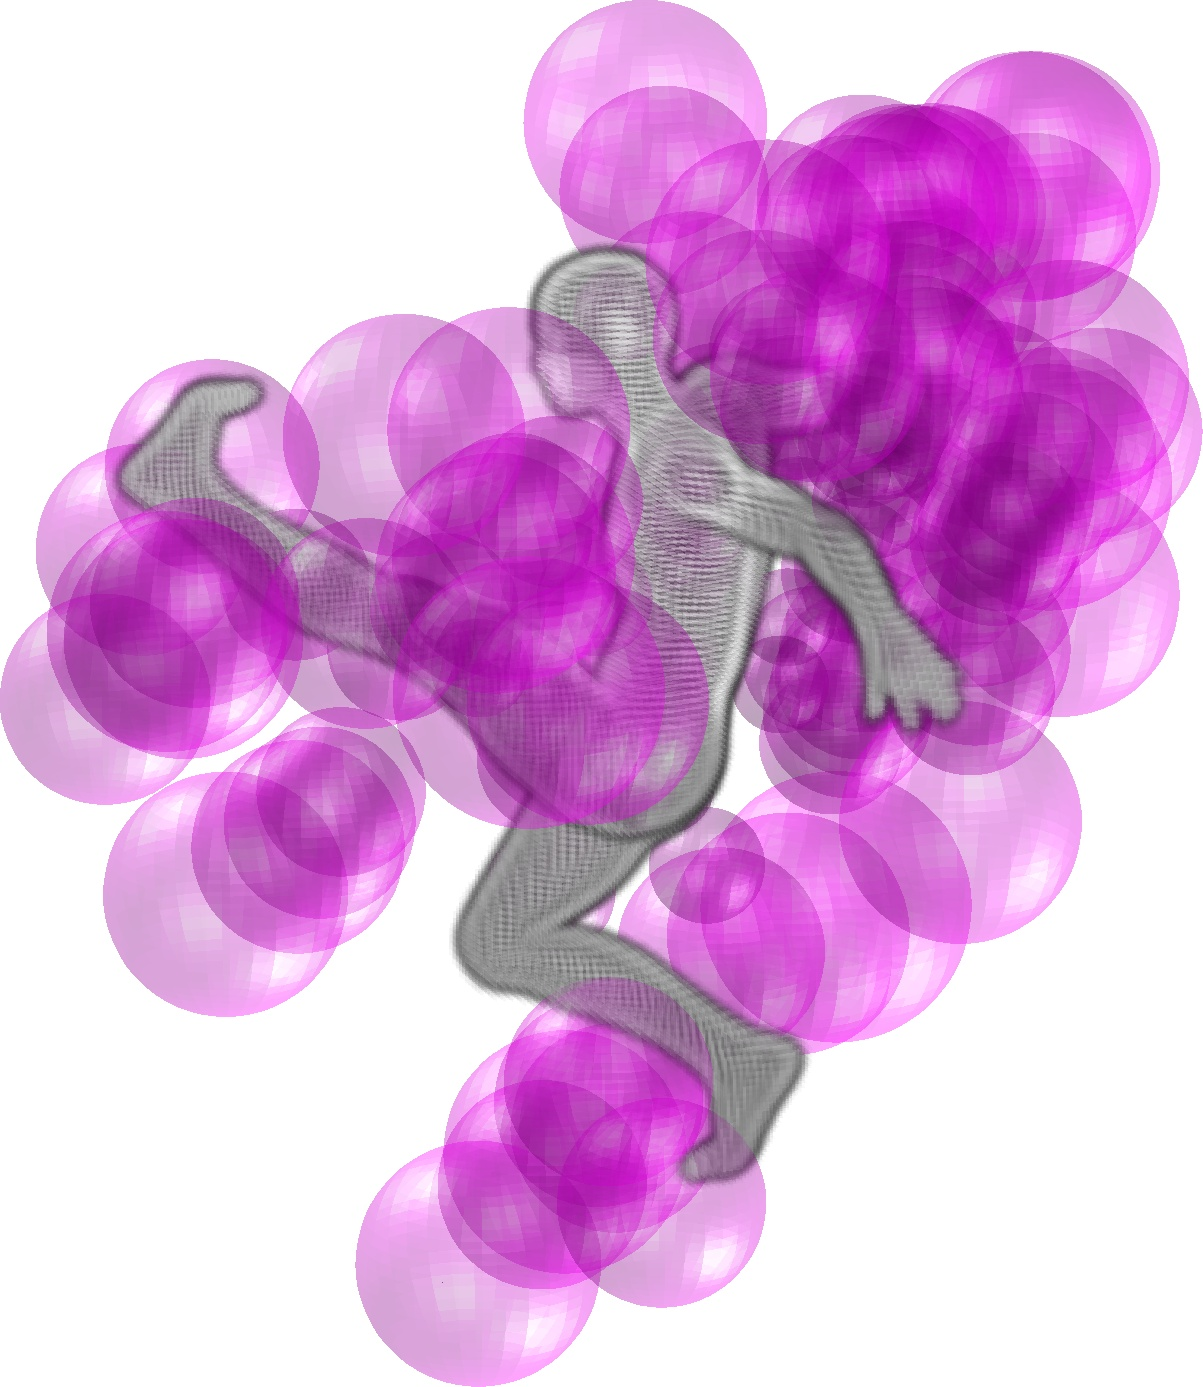
\includegraphics[width=0.155\linewidth]{./fig/eval/guy_surf.jpg}  \hspace{0mm} 
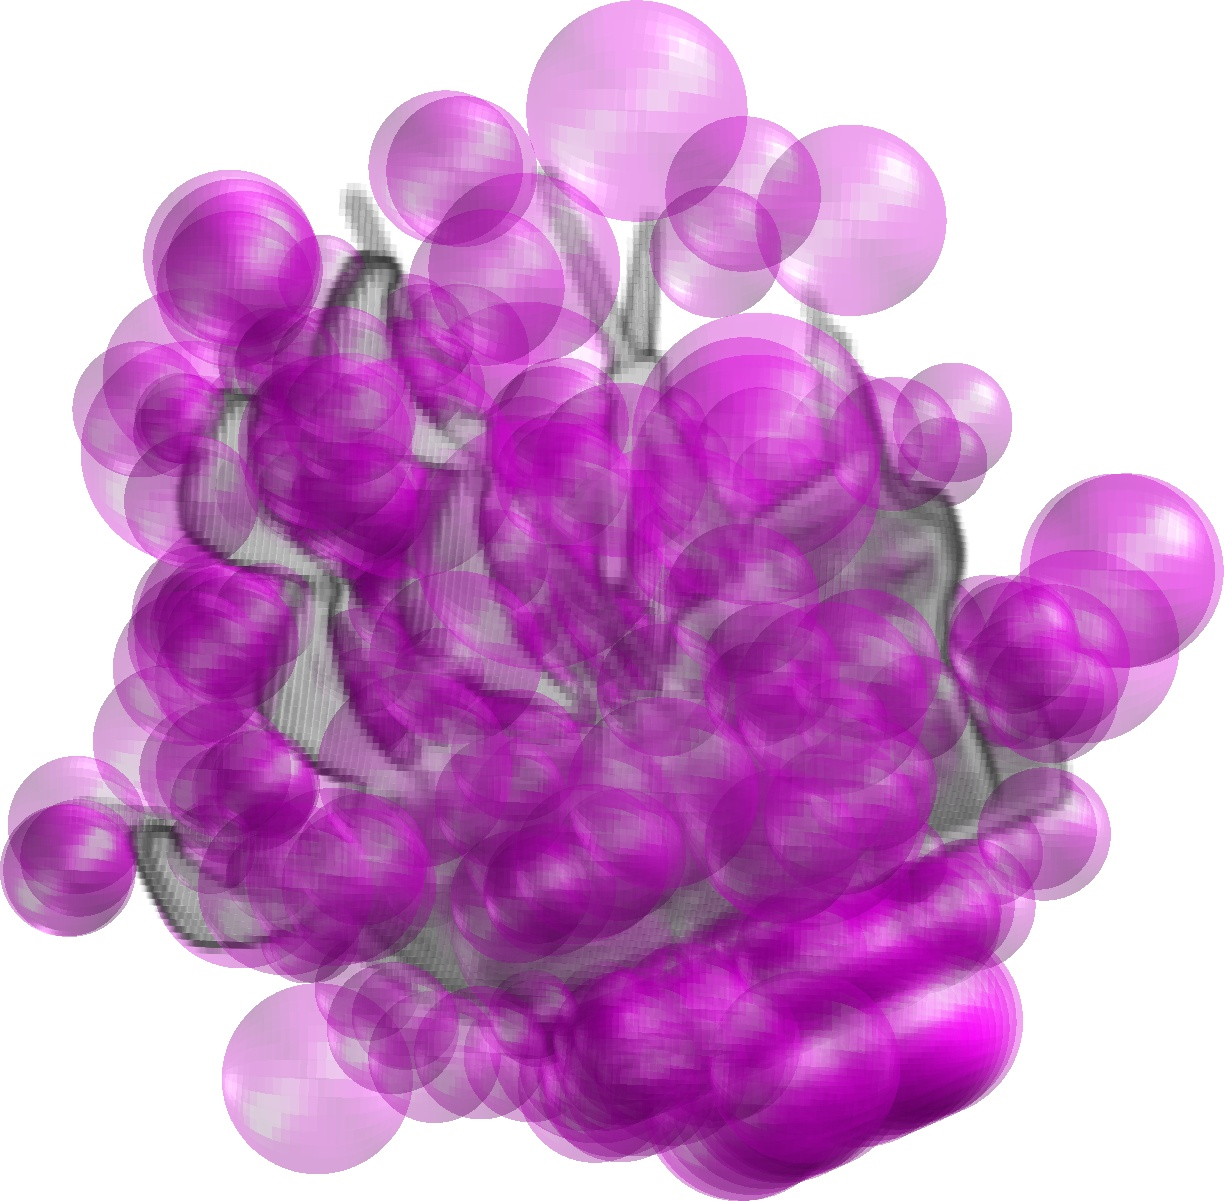
\includegraphics[width=0.175\linewidth]{./fig/eval/ship_surf.jpg} \hspace{0mm} 
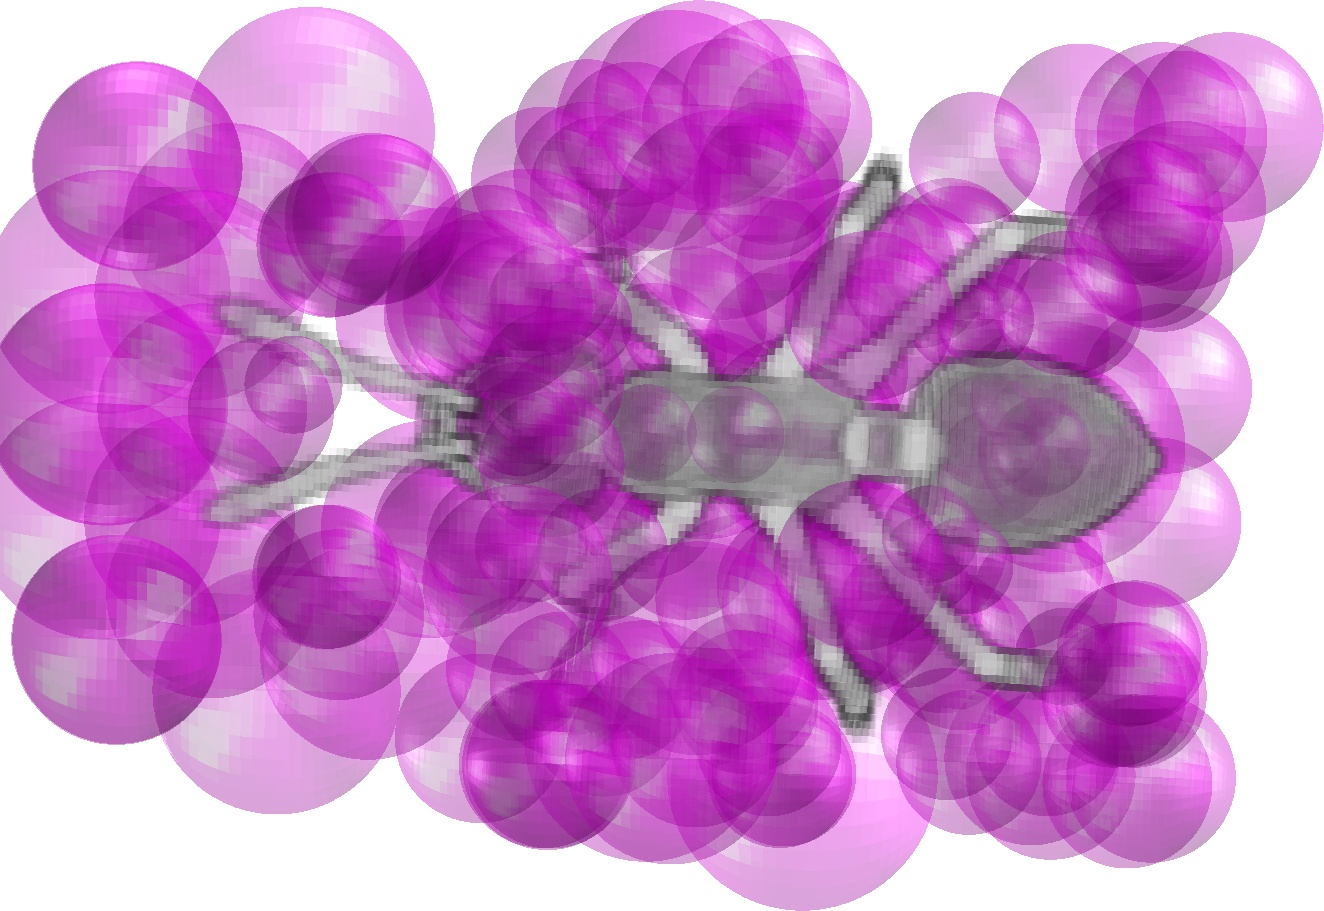
\includegraphics[width=0.175\linewidth]{./fig/eval/ant_surf.jpg} 
} \vspace{-4mm}
\\
% HARRIS
\subfloat{ 
\label{fig:mesh:harris}
\makebox[0.15\linewidth]{\raisebox{0.07\linewidth}{(d) Harris}}
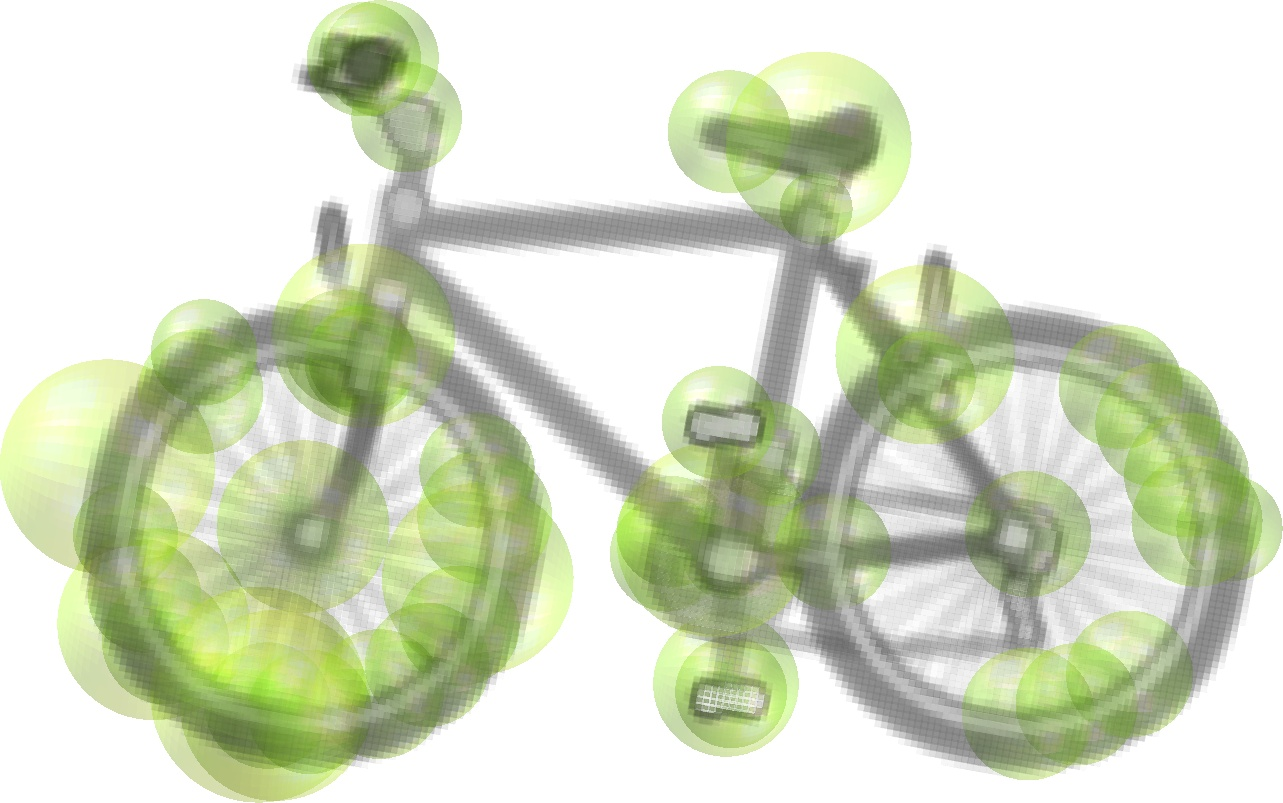
\includegraphics[width=0.175\linewidth]{./fig/eval/cycle_harris.jpg} \hspace{0mm} 
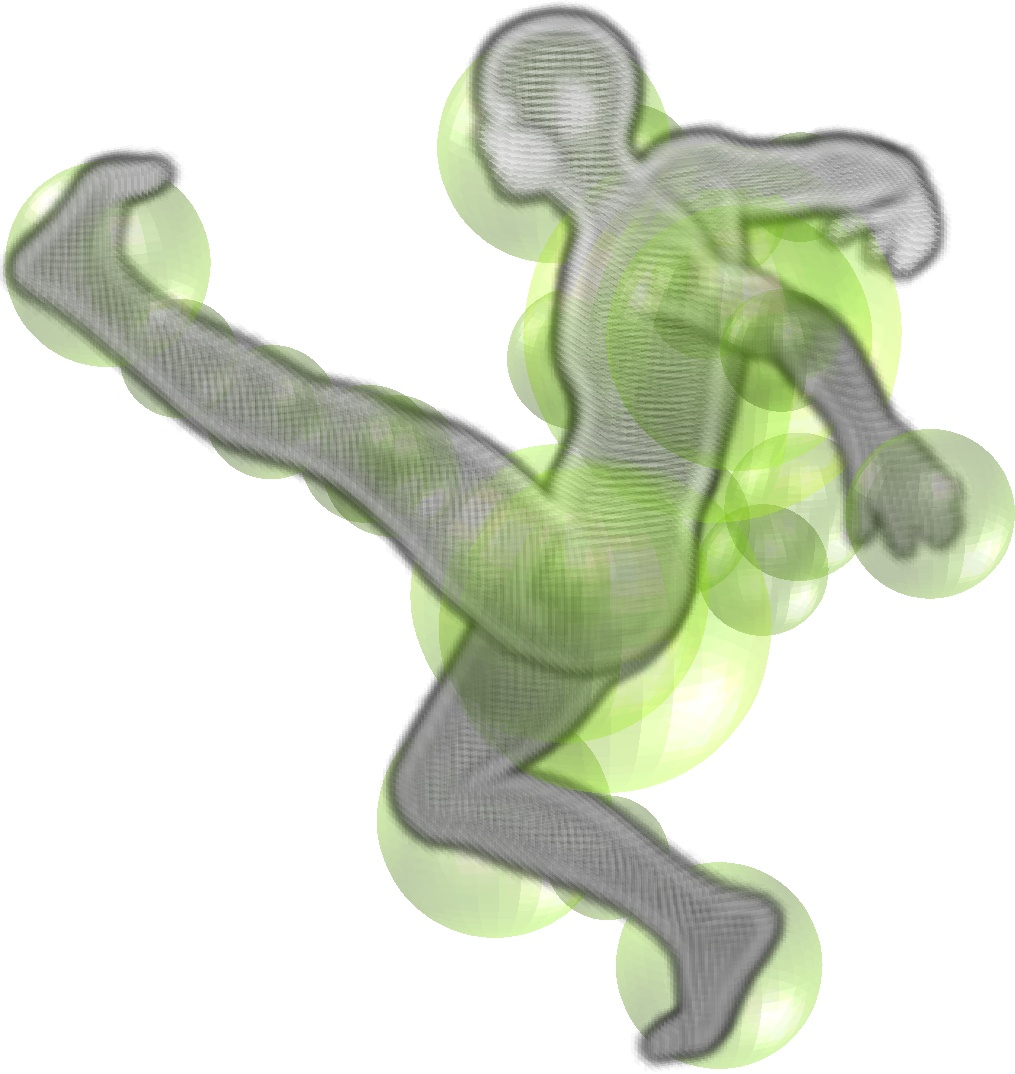
\includegraphics[width=0.155\linewidth]{./fig/eval/guy_harris.jpg}  \hspace{0mm} 
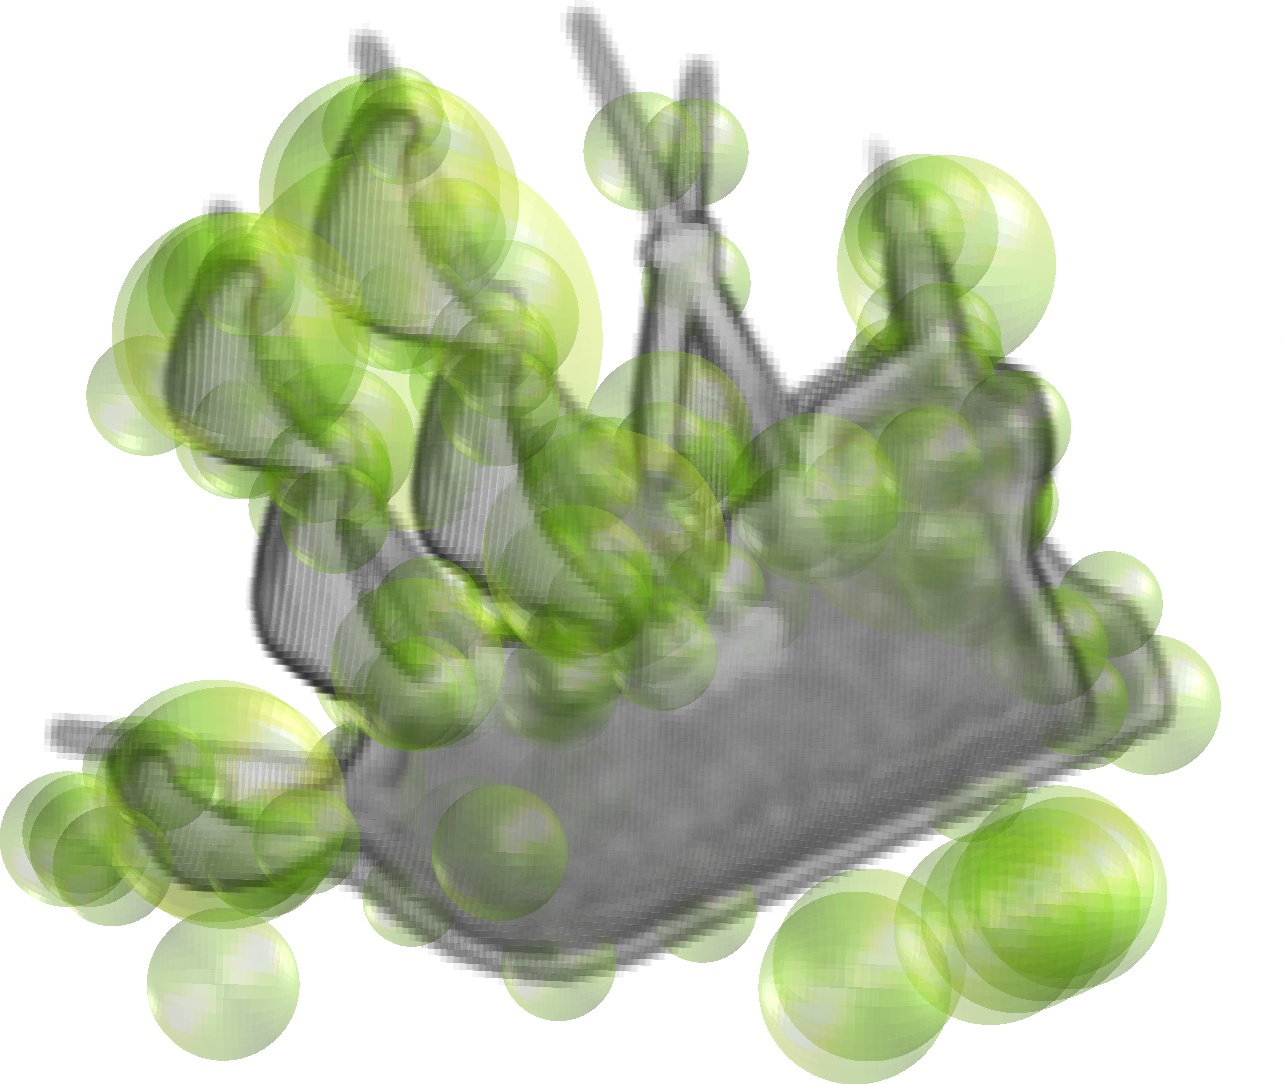
\includegraphics[width=0.175\linewidth]{./fig/eval/ship_harris.jpg} \hspace{0mm} 
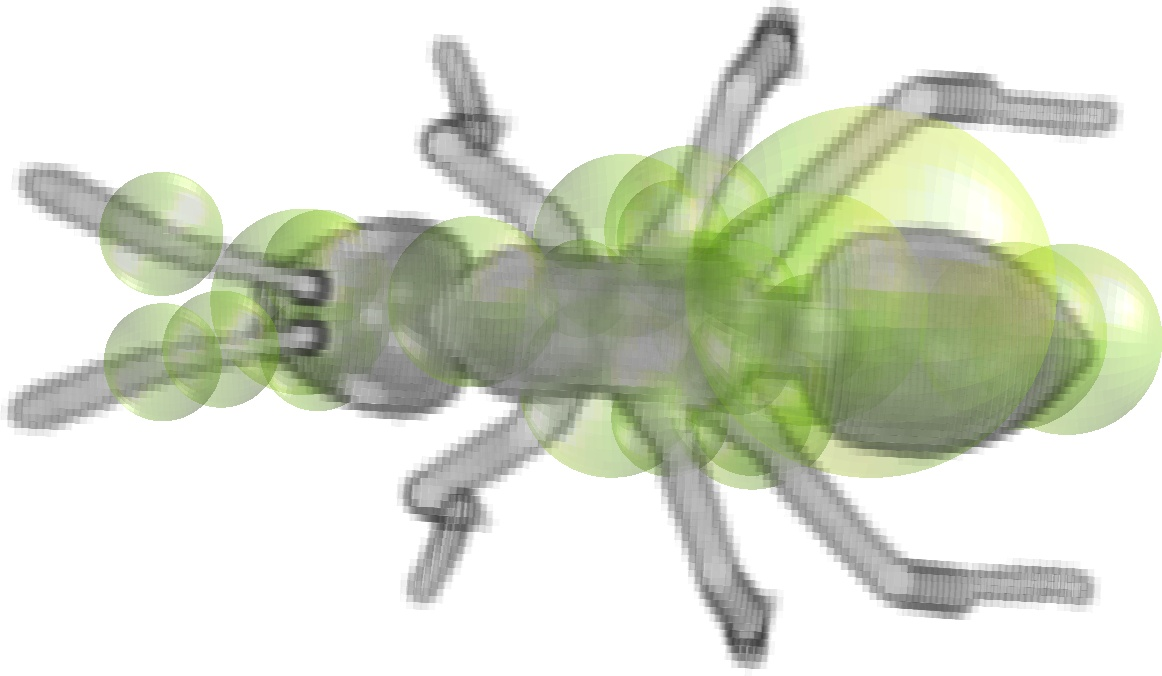
\includegraphics[width=0.175\linewidth]{./fig/eval/ant_harris.jpg} 
} \vspace{-4mm}
\\
% HESSIAN
\subfloat{ 
\label{fig:mesh:hessian}
\makebox[0.15\linewidth]{\raisebox{0.07\linewidth}{(e) DoH}} 
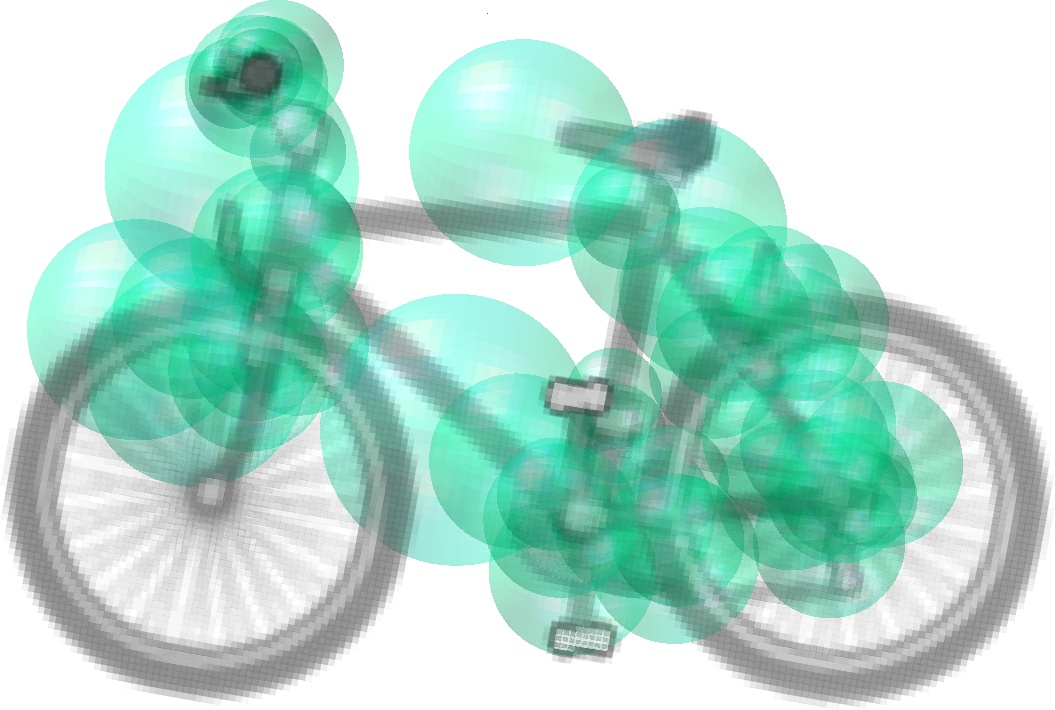
\includegraphics[width=0.175\linewidth]{./fig/eval/cycle_hessian.jpg} \hspace{0mm} 
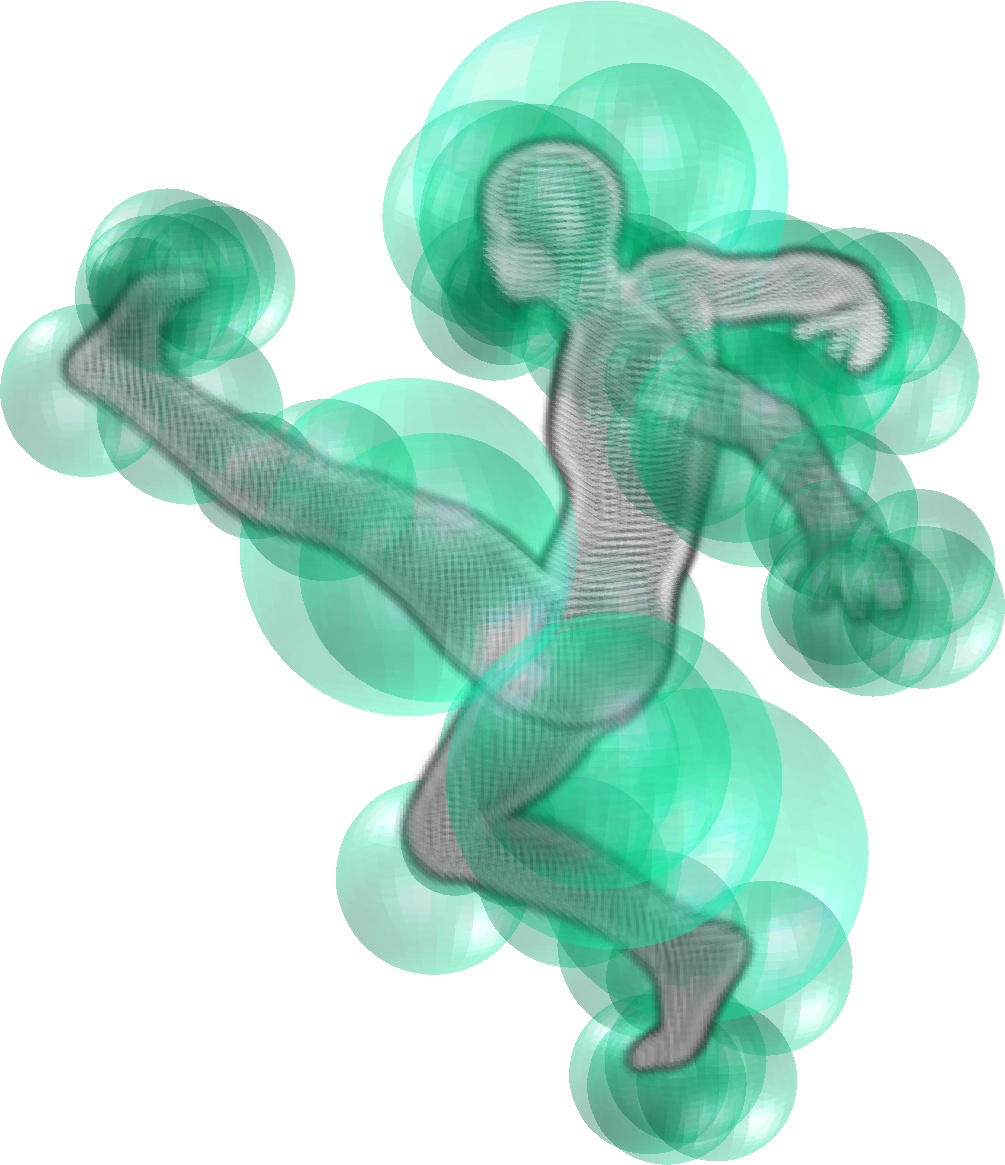
\includegraphics[width=0.155\linewidth]{./fig/eval/guy_hessian.jpg}  \hspace{0mm} 
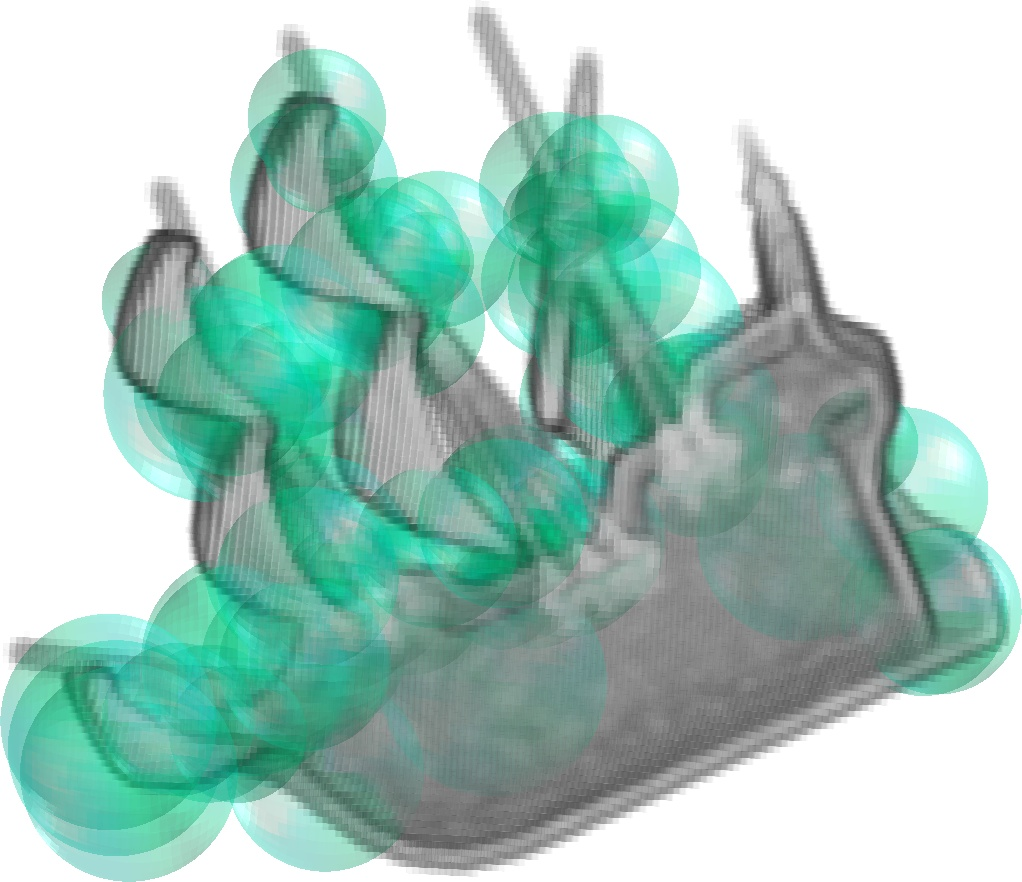
\includegraphics[width=0.175\linewidth]{./fig/eval/ship_hessian.jpg} \hspace{0mm}
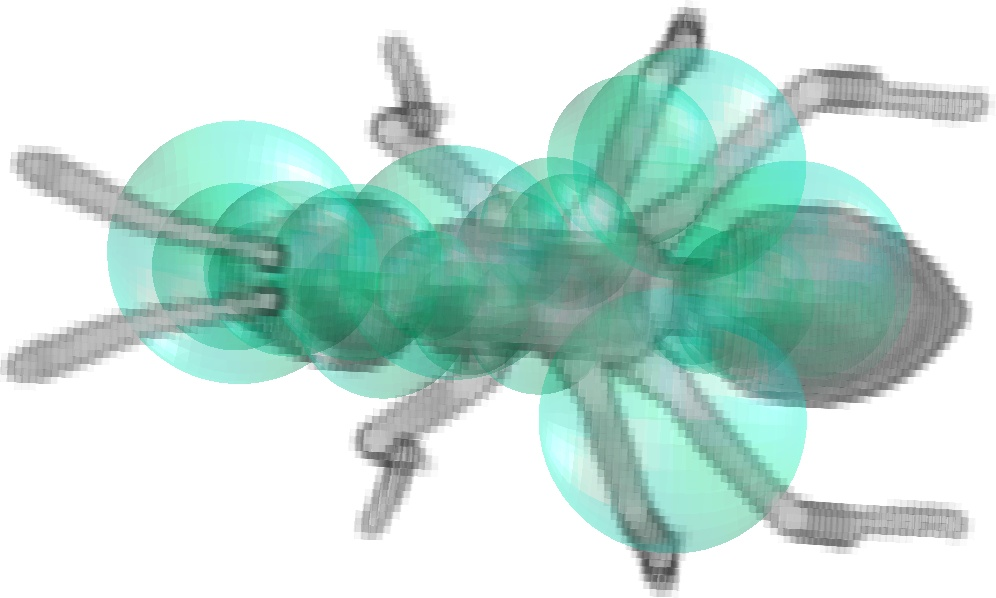
\includegraphics[width=0.175\linewidth]{./fig/eval/ant_hessian.jpg} 
} \vspace{-4mm}
\\
% FAST
\subfloat{ 
\label{fig:mesh:fast}
\makebox[0.15\linewidth]{\raisebox{0.07\linewidth}{(f) V-FAST}} 
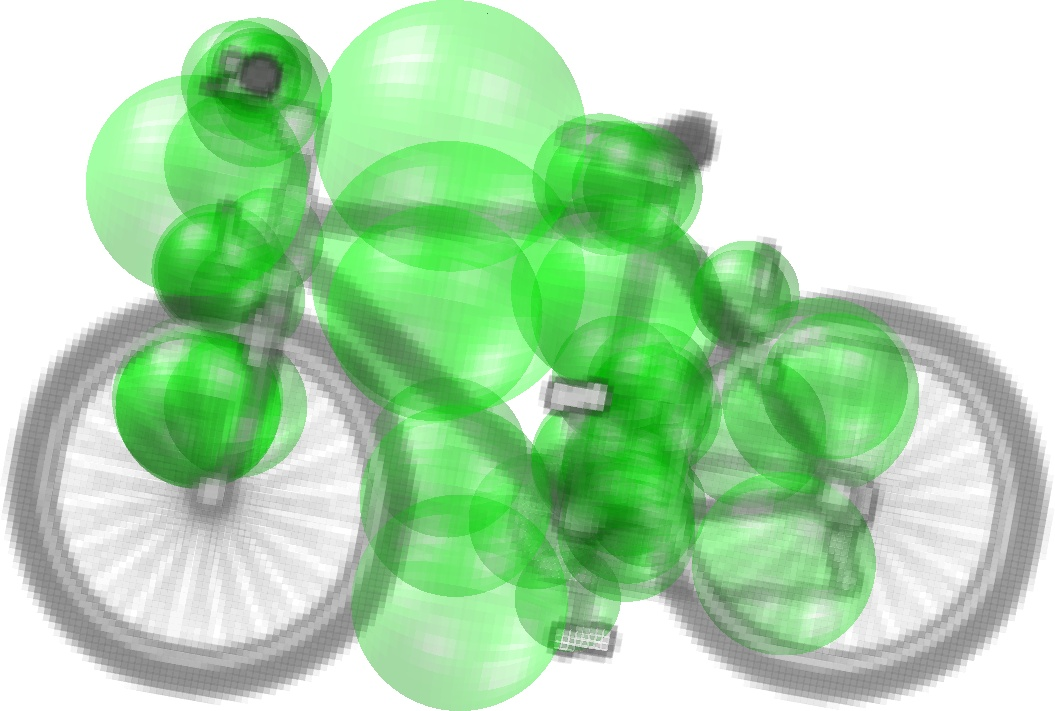
\includegraphics[width=0.175\linewidth]{./fig/eval/cycle_fast.jpg} \hspace{0mm} 
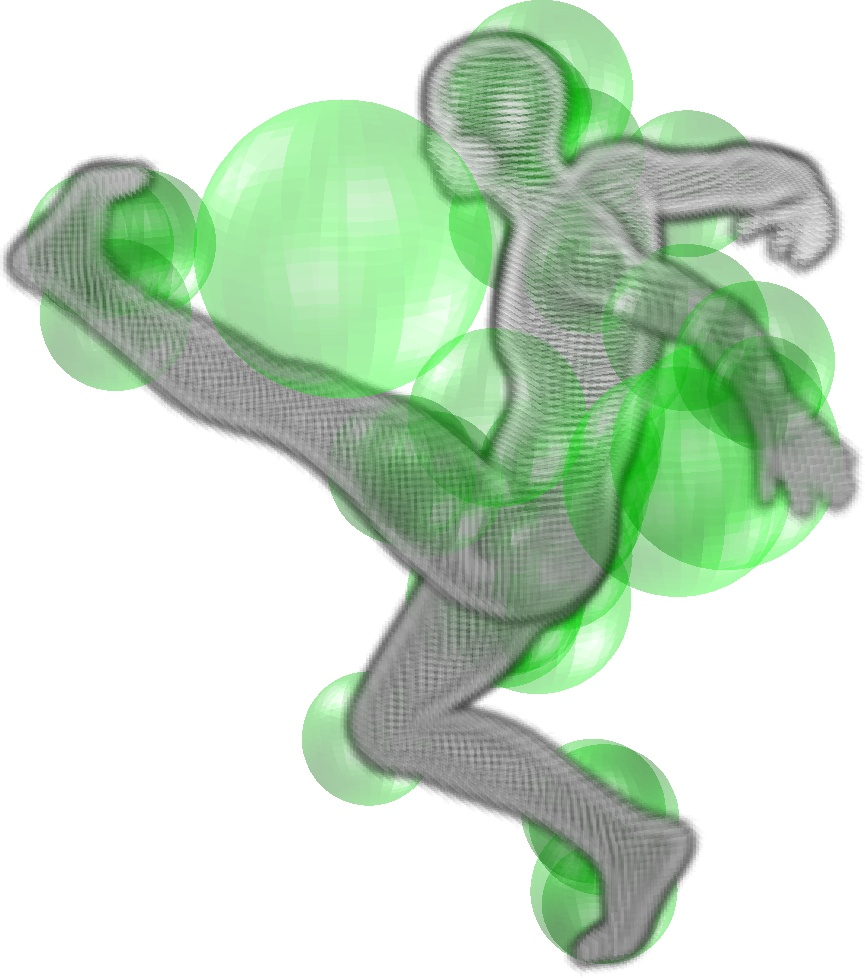
\includegraphics[width=0.155\linewidth]{./fig/eval/guy_fast.jpg}  \hspace{0mm} 
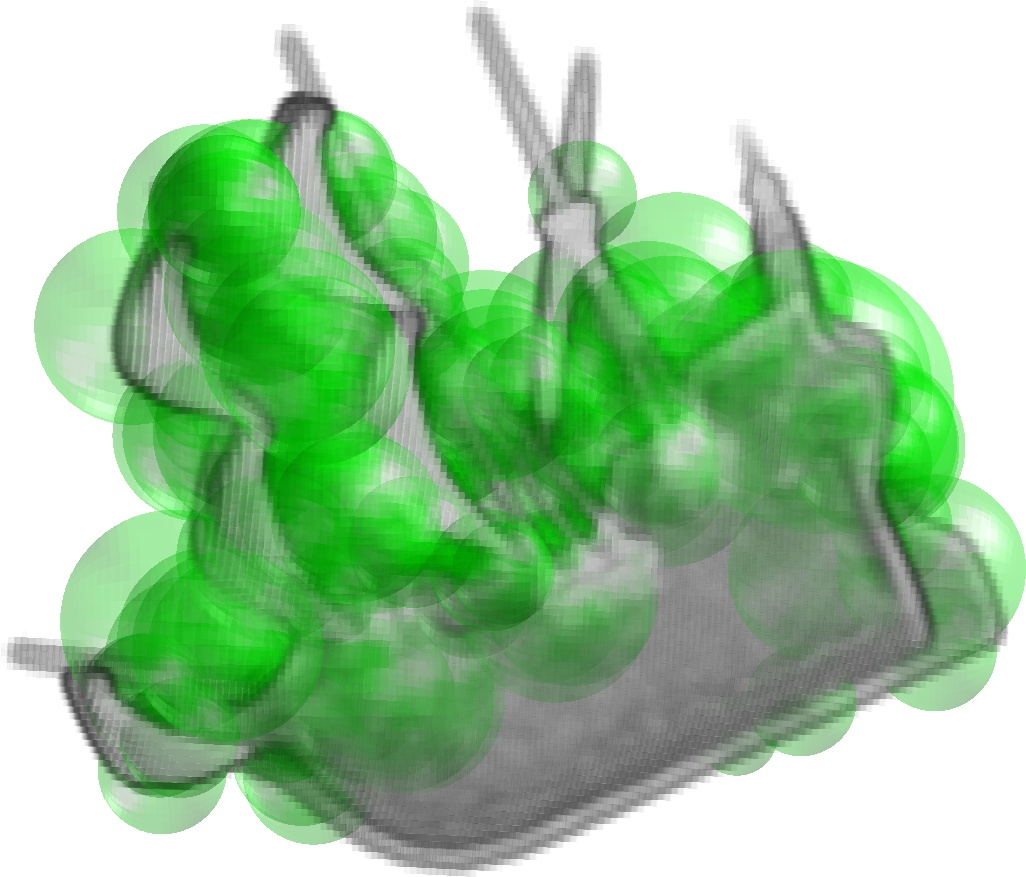
\includegraphics[width=0.175\linewidth]{./fig/eval/ship_fast.jpg} \hspace{0mm} 
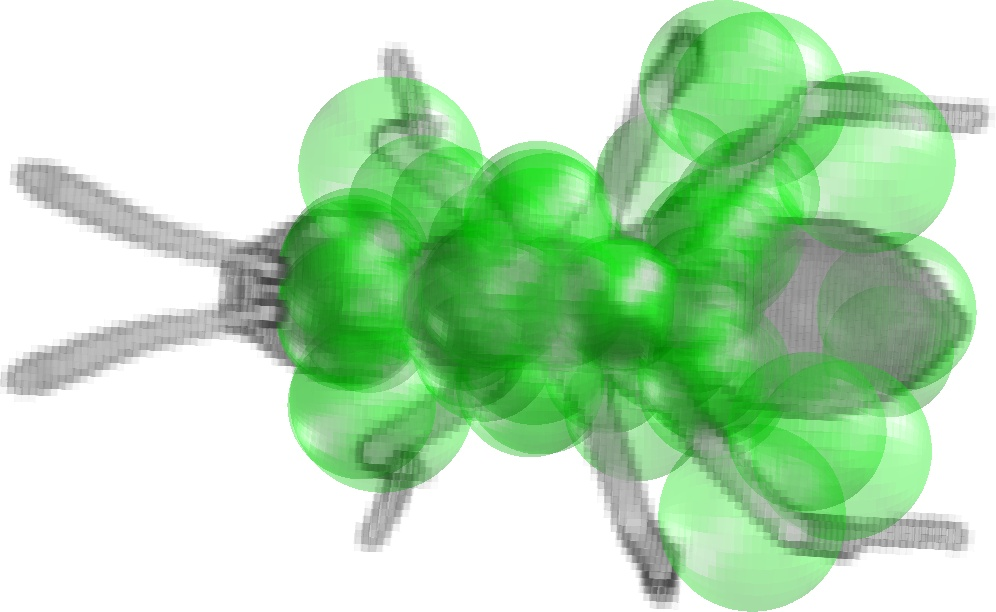
\includegraphics[width=0.175\linewidth]{./fig/eval/ant_fast.jpg} 
} \vspace{-4mm}
\\
% MSER
\subfloat{ 
\label{fig:mesh:mser}
\makebox[0.15\linewidth]{\raisebox{0.07\linewidth}{(g) MSER}}
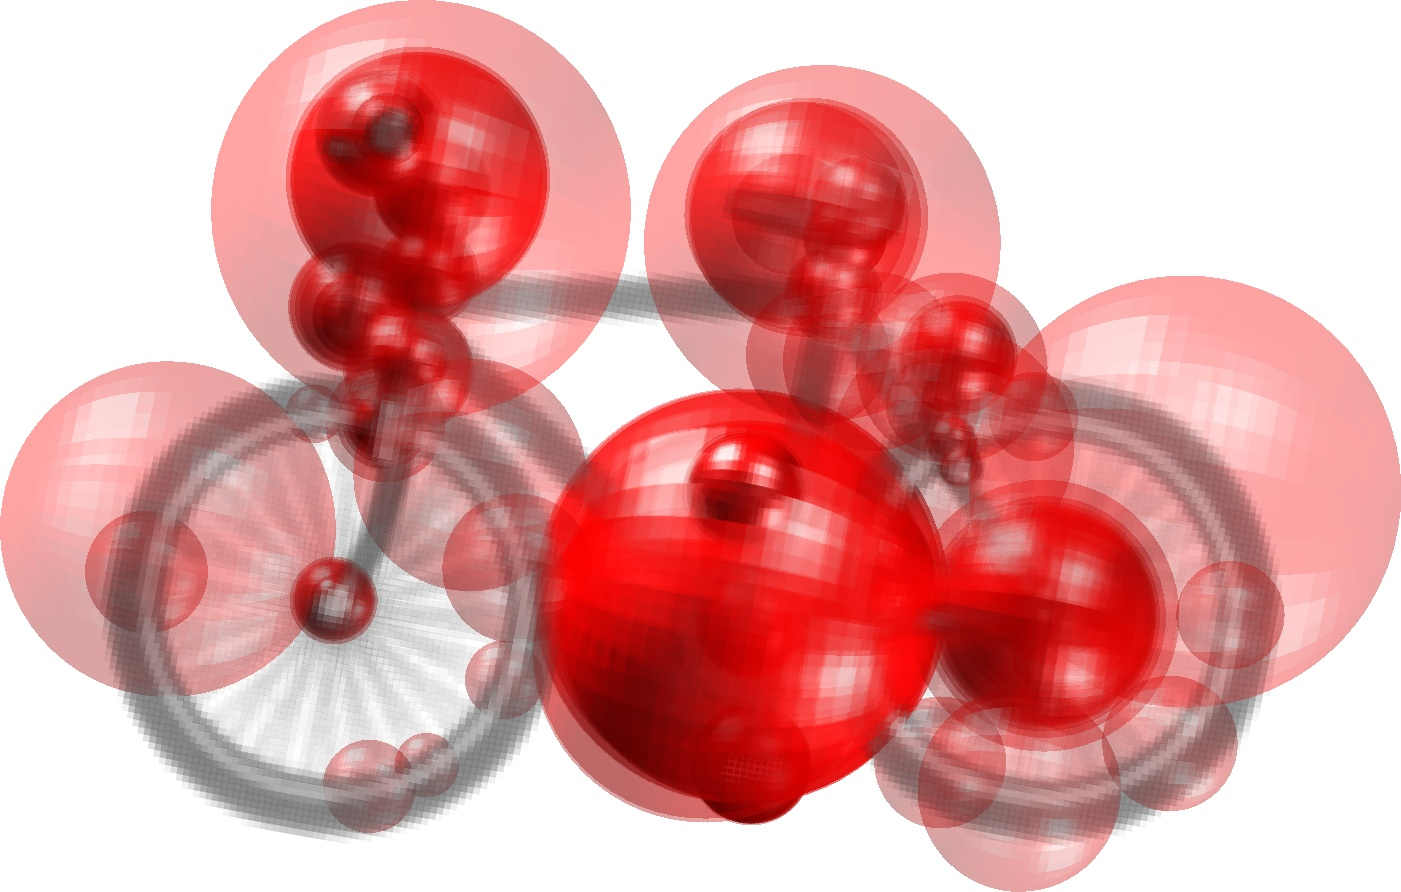
\includegraphics[width=0.175\linewidth]{./fig/eval/cycle_mser.jpg} \hspace{0mm}
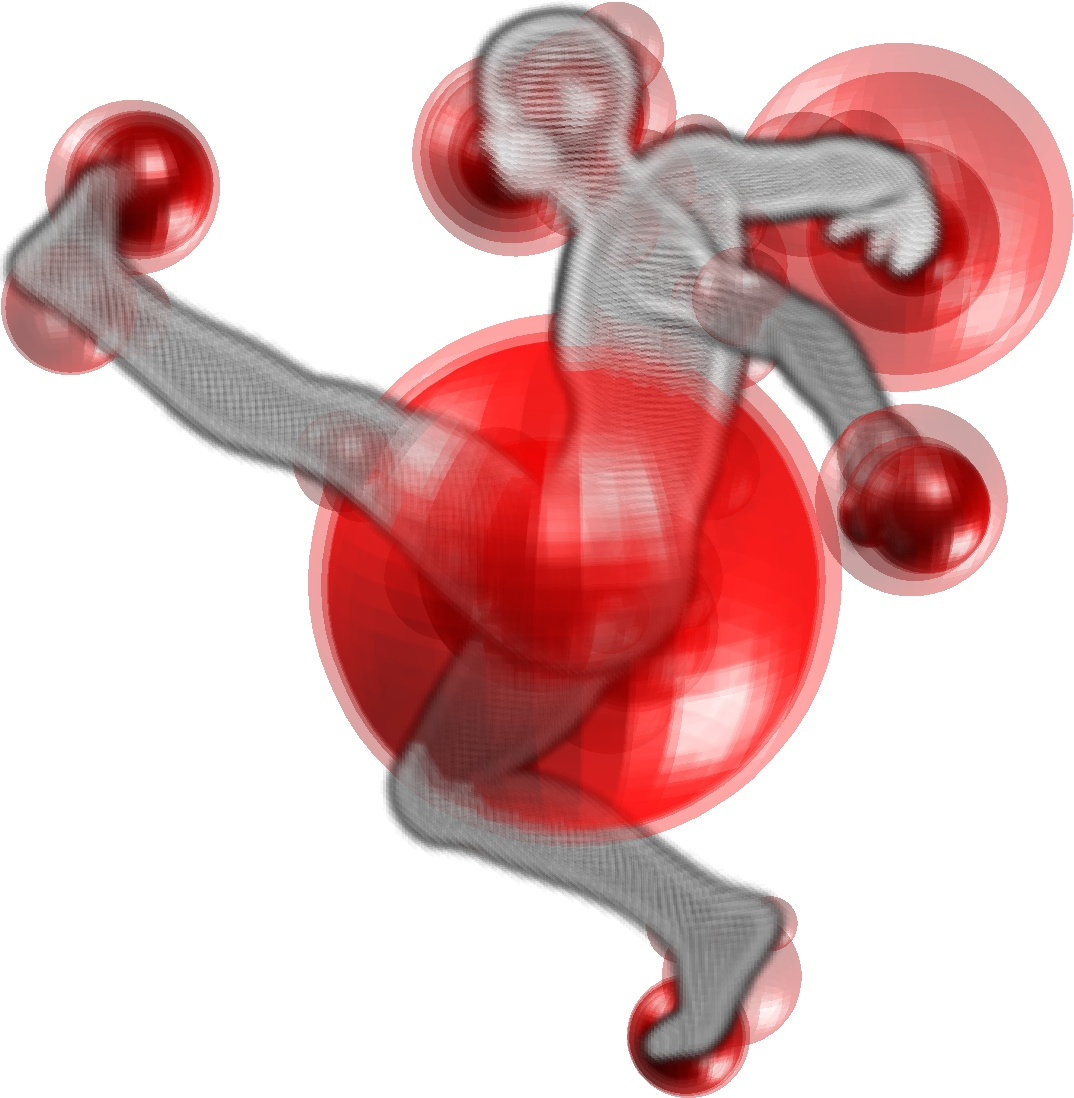
\includegraphics[width=0.155\linewidth]{./fig/eval/guy_mser.jpg}  \hspace{0mm} 
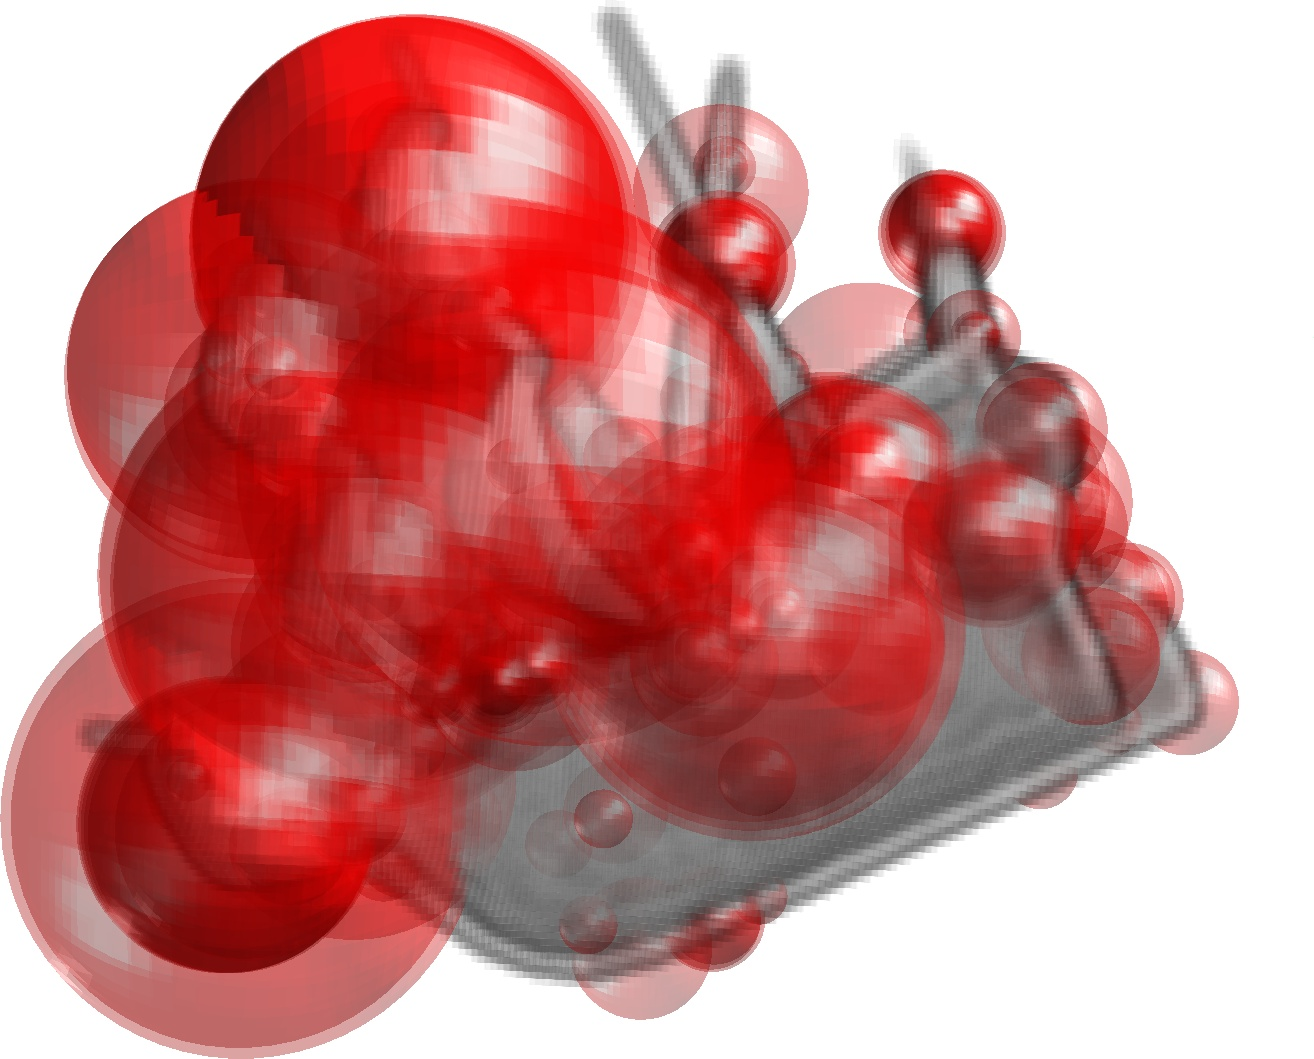
\includegraphics[width=0.175\linewidth]{./fig/eval/ship_mser.jpg} \hspace{0mm}
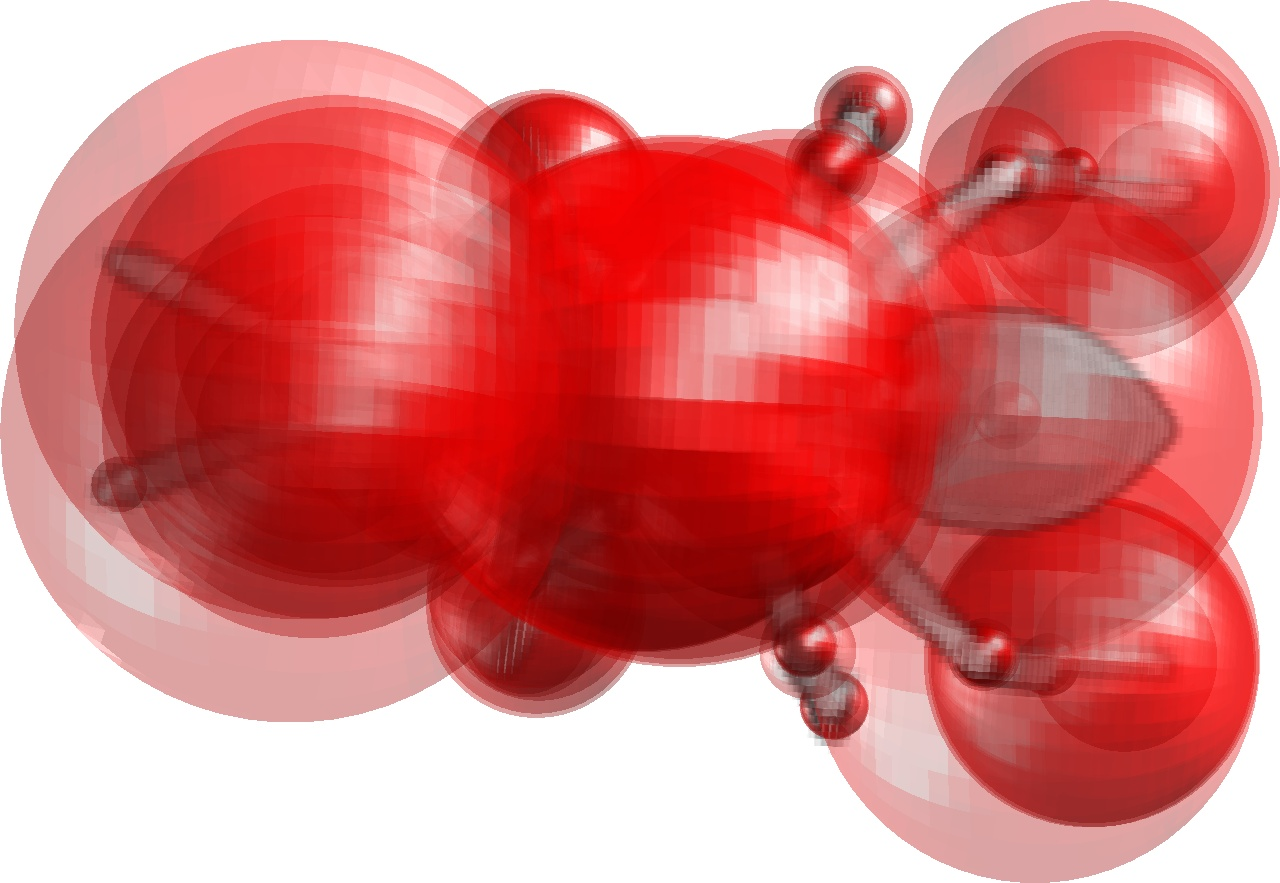
\includegraphics[width=0.175\linewidth]{./fig/eval/ant_mser.jpg} 
} 
\caption{(a) Sample point clouds obtained from the \textbf{Mesh} dataset, (b) DoG, (c) SURF (d) Harris, (e) DoH, (f) V-FAST and (g) MSER, visualized on the voxelized data. The color spheres represent the positions and relative scales of the detected interest points.}
\label{fig:mesh}
\end{figure*}
